\subsection{Ensemble methods}

\vspace{0.2cm}
\noindent
\textbf{Random forest \& bagging}

We improved the tree-based models using bagging with 500 trees and random forest, selecting the best number of predictors (\textit{m}) from the full set of \textit{p} predictors.

In \Fig~\ref{fig:m_best_for_500_plot} we can see the trend of the test and the out-of-bag error rates as \textit{m} increases.

\begin{figure}[h]
	\centering
	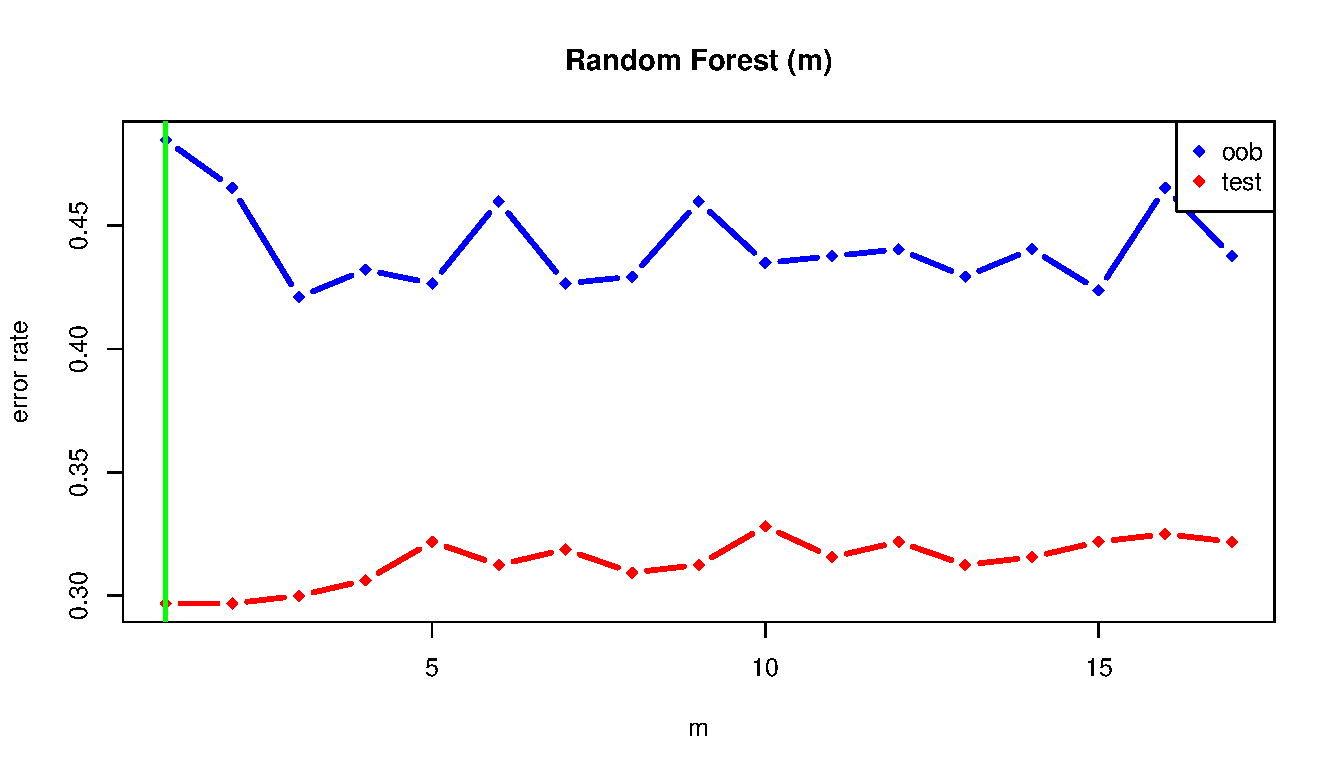
\includegraphics[width=0.5\linewidth]{ImageFiles/Classification/Trees/m_best_for_500_plot.pdf}
	\caption{Plot of the error rate trends in random forest for varying values of \textit{m} (test: red, out-of-bag: blue).}
	\label{fig:m_best_for_500_plot}
\end{figure}

Once the best \textit{m} value for the random forest was obtained ($m = 1$), we compared the bagging model with the random forest model using that particular value of \textit{m}, while keeping all other parameters the same.
In \Fig~\ref{fig:best_for_500_plot} and \Fig~\ref{fig:bagg_500_plot} are presented the individual performances of the random forest and the bagging technique respectively. 
In \Fig~\ref{fig:vs_bagg_for_500_plot} we can see that random forest performs slightly better than bagging. 

\begin{figure}[h]
	\centering
	\hfill
	\begin{subfigure}{.5\textwidth}
		\centering
		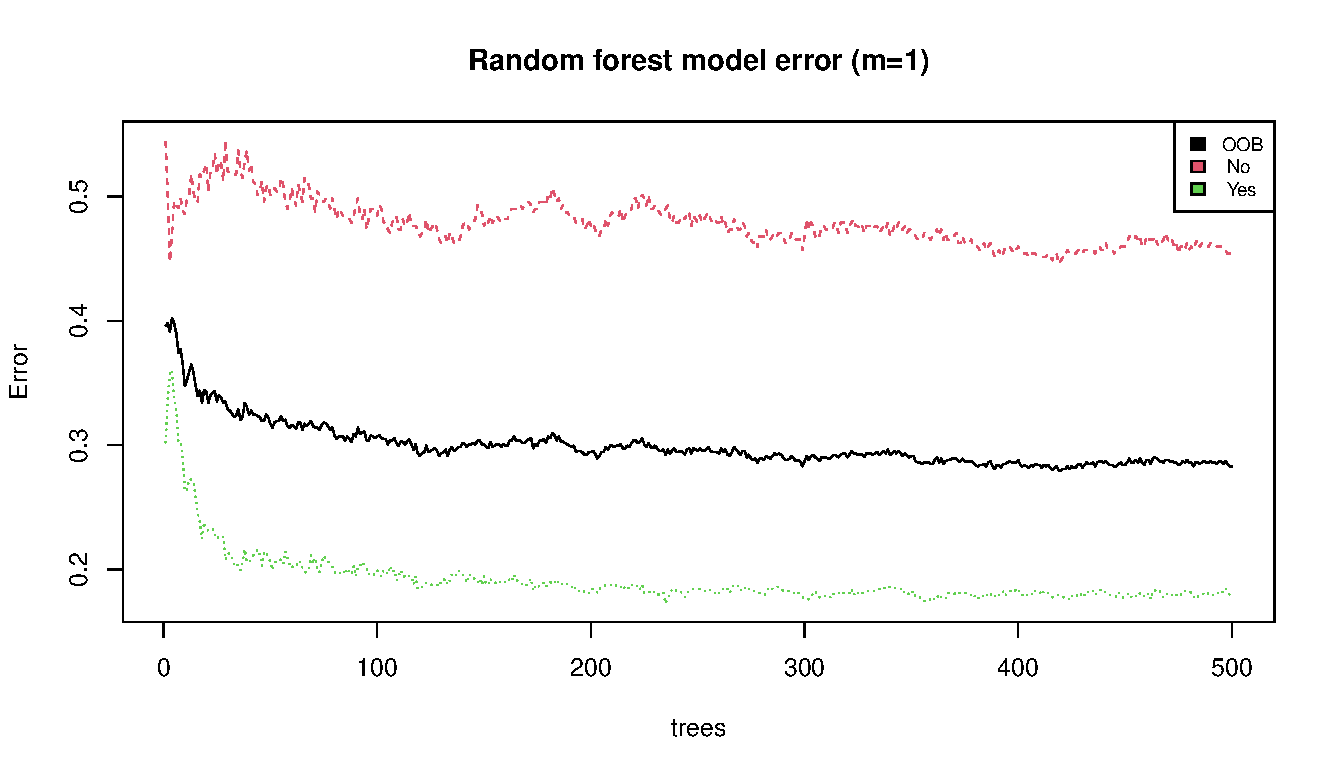
\includegraphics[width=0.7\linewidth]{ImageFiles/Classification/Trees/best_for_500_plot.pdf}
		\caption{}
		\label{fig:best_for_500_plot}
	\end{subfigure}%
	\hfill
	\begin{subfigure}{.5\textwidth}
		\centering
		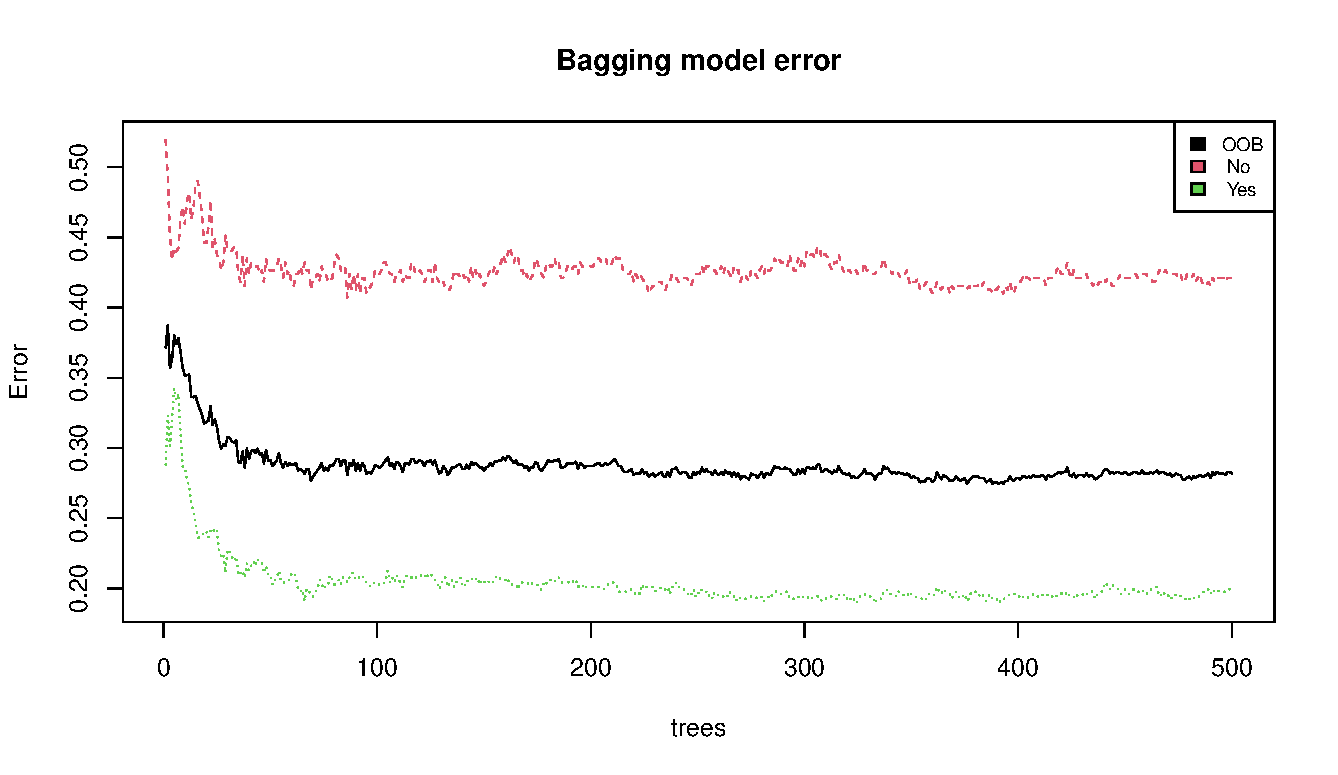
\includegraphics[width=0.7\linewidth]{ImageFiles/Classification/Trees/bagg_500_plot.pdf}
		\caption{}
		\label{fig:bagg_500_plot}
	\end{subfigure}
	\begin{subfigure}{.5\textwidth}
		\centering
		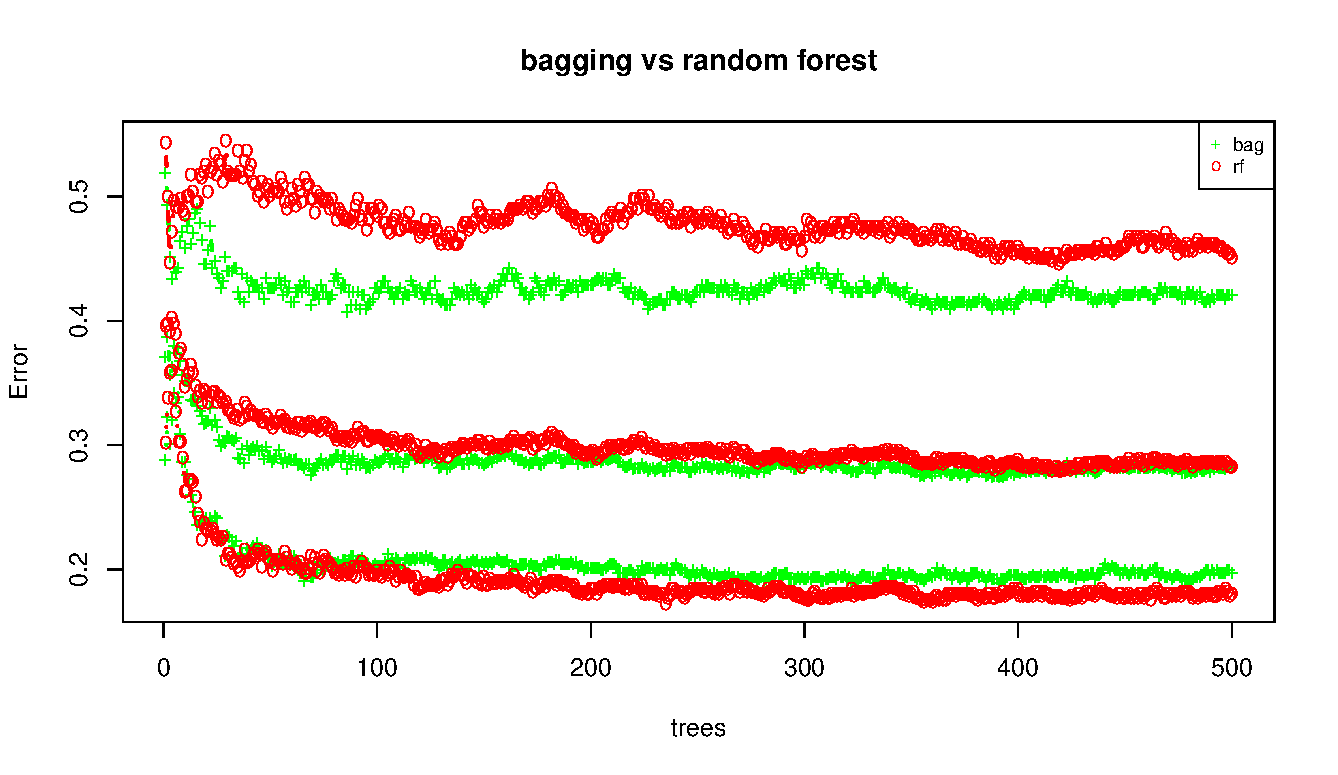
\includegraphics[width=0.7\linewidth]{ImageFiles/Classification/Trees/vs_bagg_for_500_plot.pdf}
		\caption{}
		\label{fig:vs_bagg_for_500_plot}
	\end{subfigure}
	\caption{Comparison between random forest and bagging performances as the number of trees increases. (a) Random forest error rate trends (red: no, black: out-of-bag, green: yes). (b) Bagging error rate trends (same legend). (c) Comparison between yes, no and out-of-bag error rates (red: random forest, green: bagging).}
	\label{fig:RFvsB}
\end{figure}

An overall summary of the importance of each predictor is obtained by using Residual Sum of Squares (RSS). \Fig~\ref{fig:best_for_500_var_imp_plot} and \Fig~\ref{fig:bagg_500_var_imp_plot} present the importance of each variable within the models. This importance can be interpreted as the degree to which the removal of a variable would negatively impact the model's performance, utilizing the mean decrease of the \textit{gini} index in relation to the maximum.

\begin{figure}[h]
	\centering
	\begin{subfigure}{.5\textwidth}
		\centering
		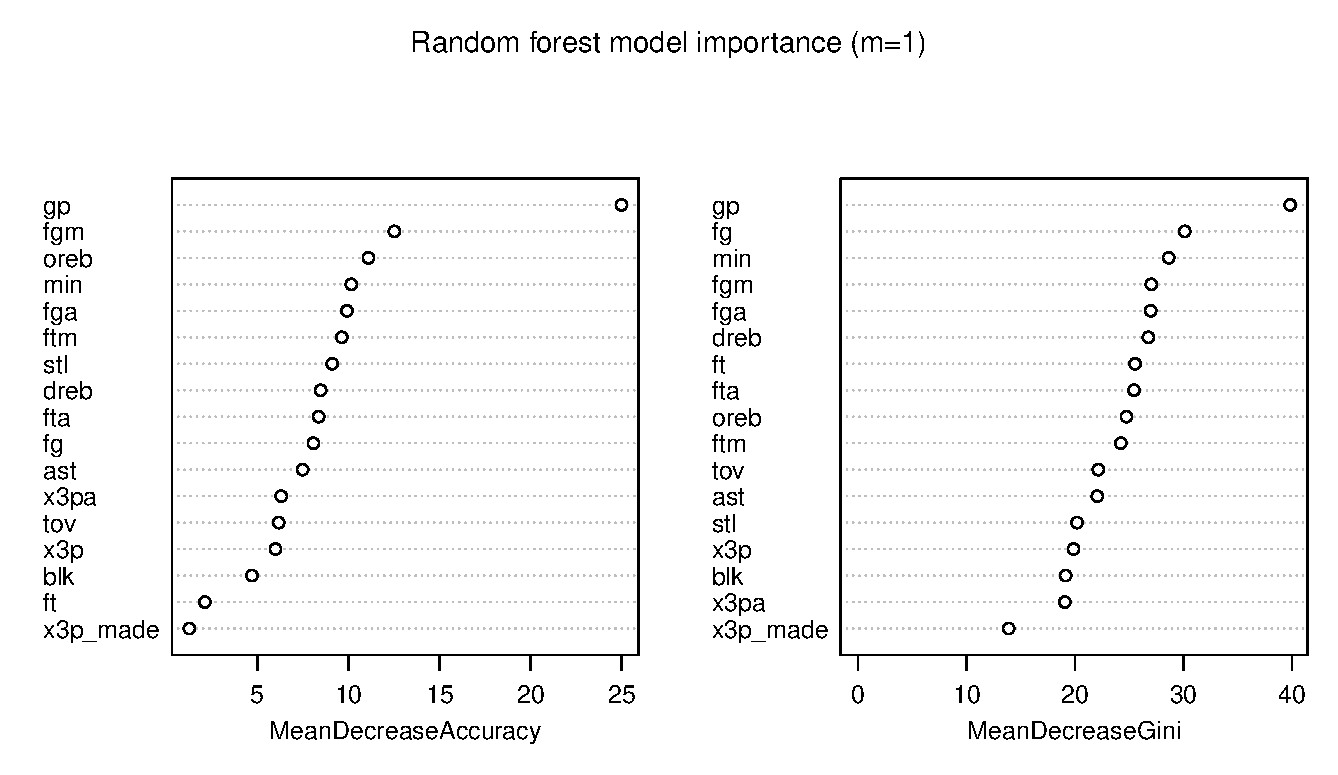
\includegraphics[width=0.9\linewidth]{ImageFiles/Classification/Trees/best_for_500_var_imp_plot.pdf}
		\caption{}
		\label{fig:best_for_500_var_imp_plot}
	\end{subfigure}%
	\hfill
	\begin{subfigure}{.5\textwidth}
		\centering
		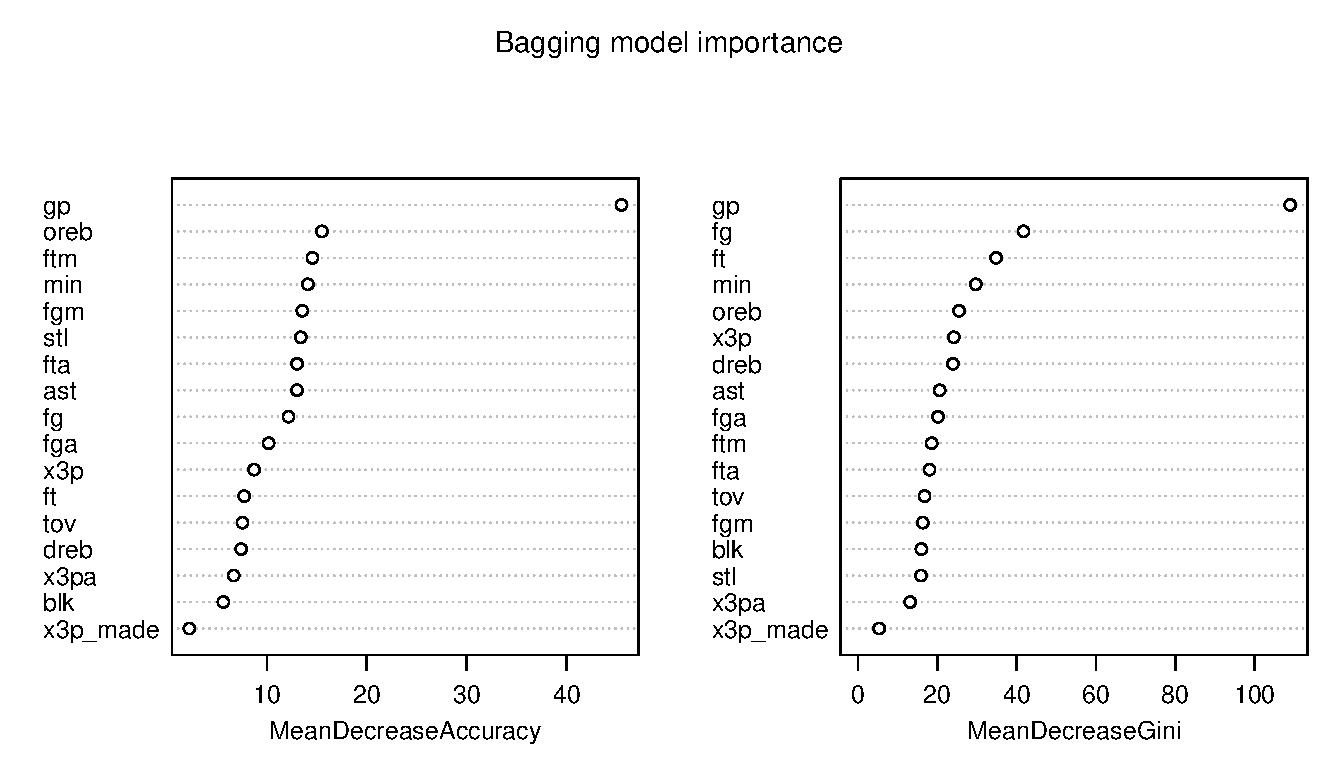
\includegraphics[width=0.9\linewidth]{ImageFiles/Classification/Trees/bagg_500_var_imp_plot.pdf}
		\caption{}
		\label{fig:bagg_500_var_imp_plot}
	\end{subfigure}
	\caption{Plot of the importance of all the variables. (a) Importance in the random forest model. (b) Importance in the bagging model.}
	\label{fig:ImpVar}
\end{figure}

As in the classification trees, the ``GP'' regressor resulted to be the most important one.

\vspace{0.2cm}
\noindent
\textbf{Boosting}

Since the main goal of this section is to find the model that best explain our data, we tried to improve the performance by using boosting in conjunction with cross-validation, even at the cost of losing interpretability. 

After applying the boosting technique with 5000 iterations, the importance of each variable in the dataset is shown in \Fig~\ref{fig:boost_4_rel_inf}. The figure showcases the model from the iteration that yielded the lowest cross-validation error.

\begin{figure}[h]
	\centering
	\begin{subfigure}{0.5\textwidth}
		\centering
		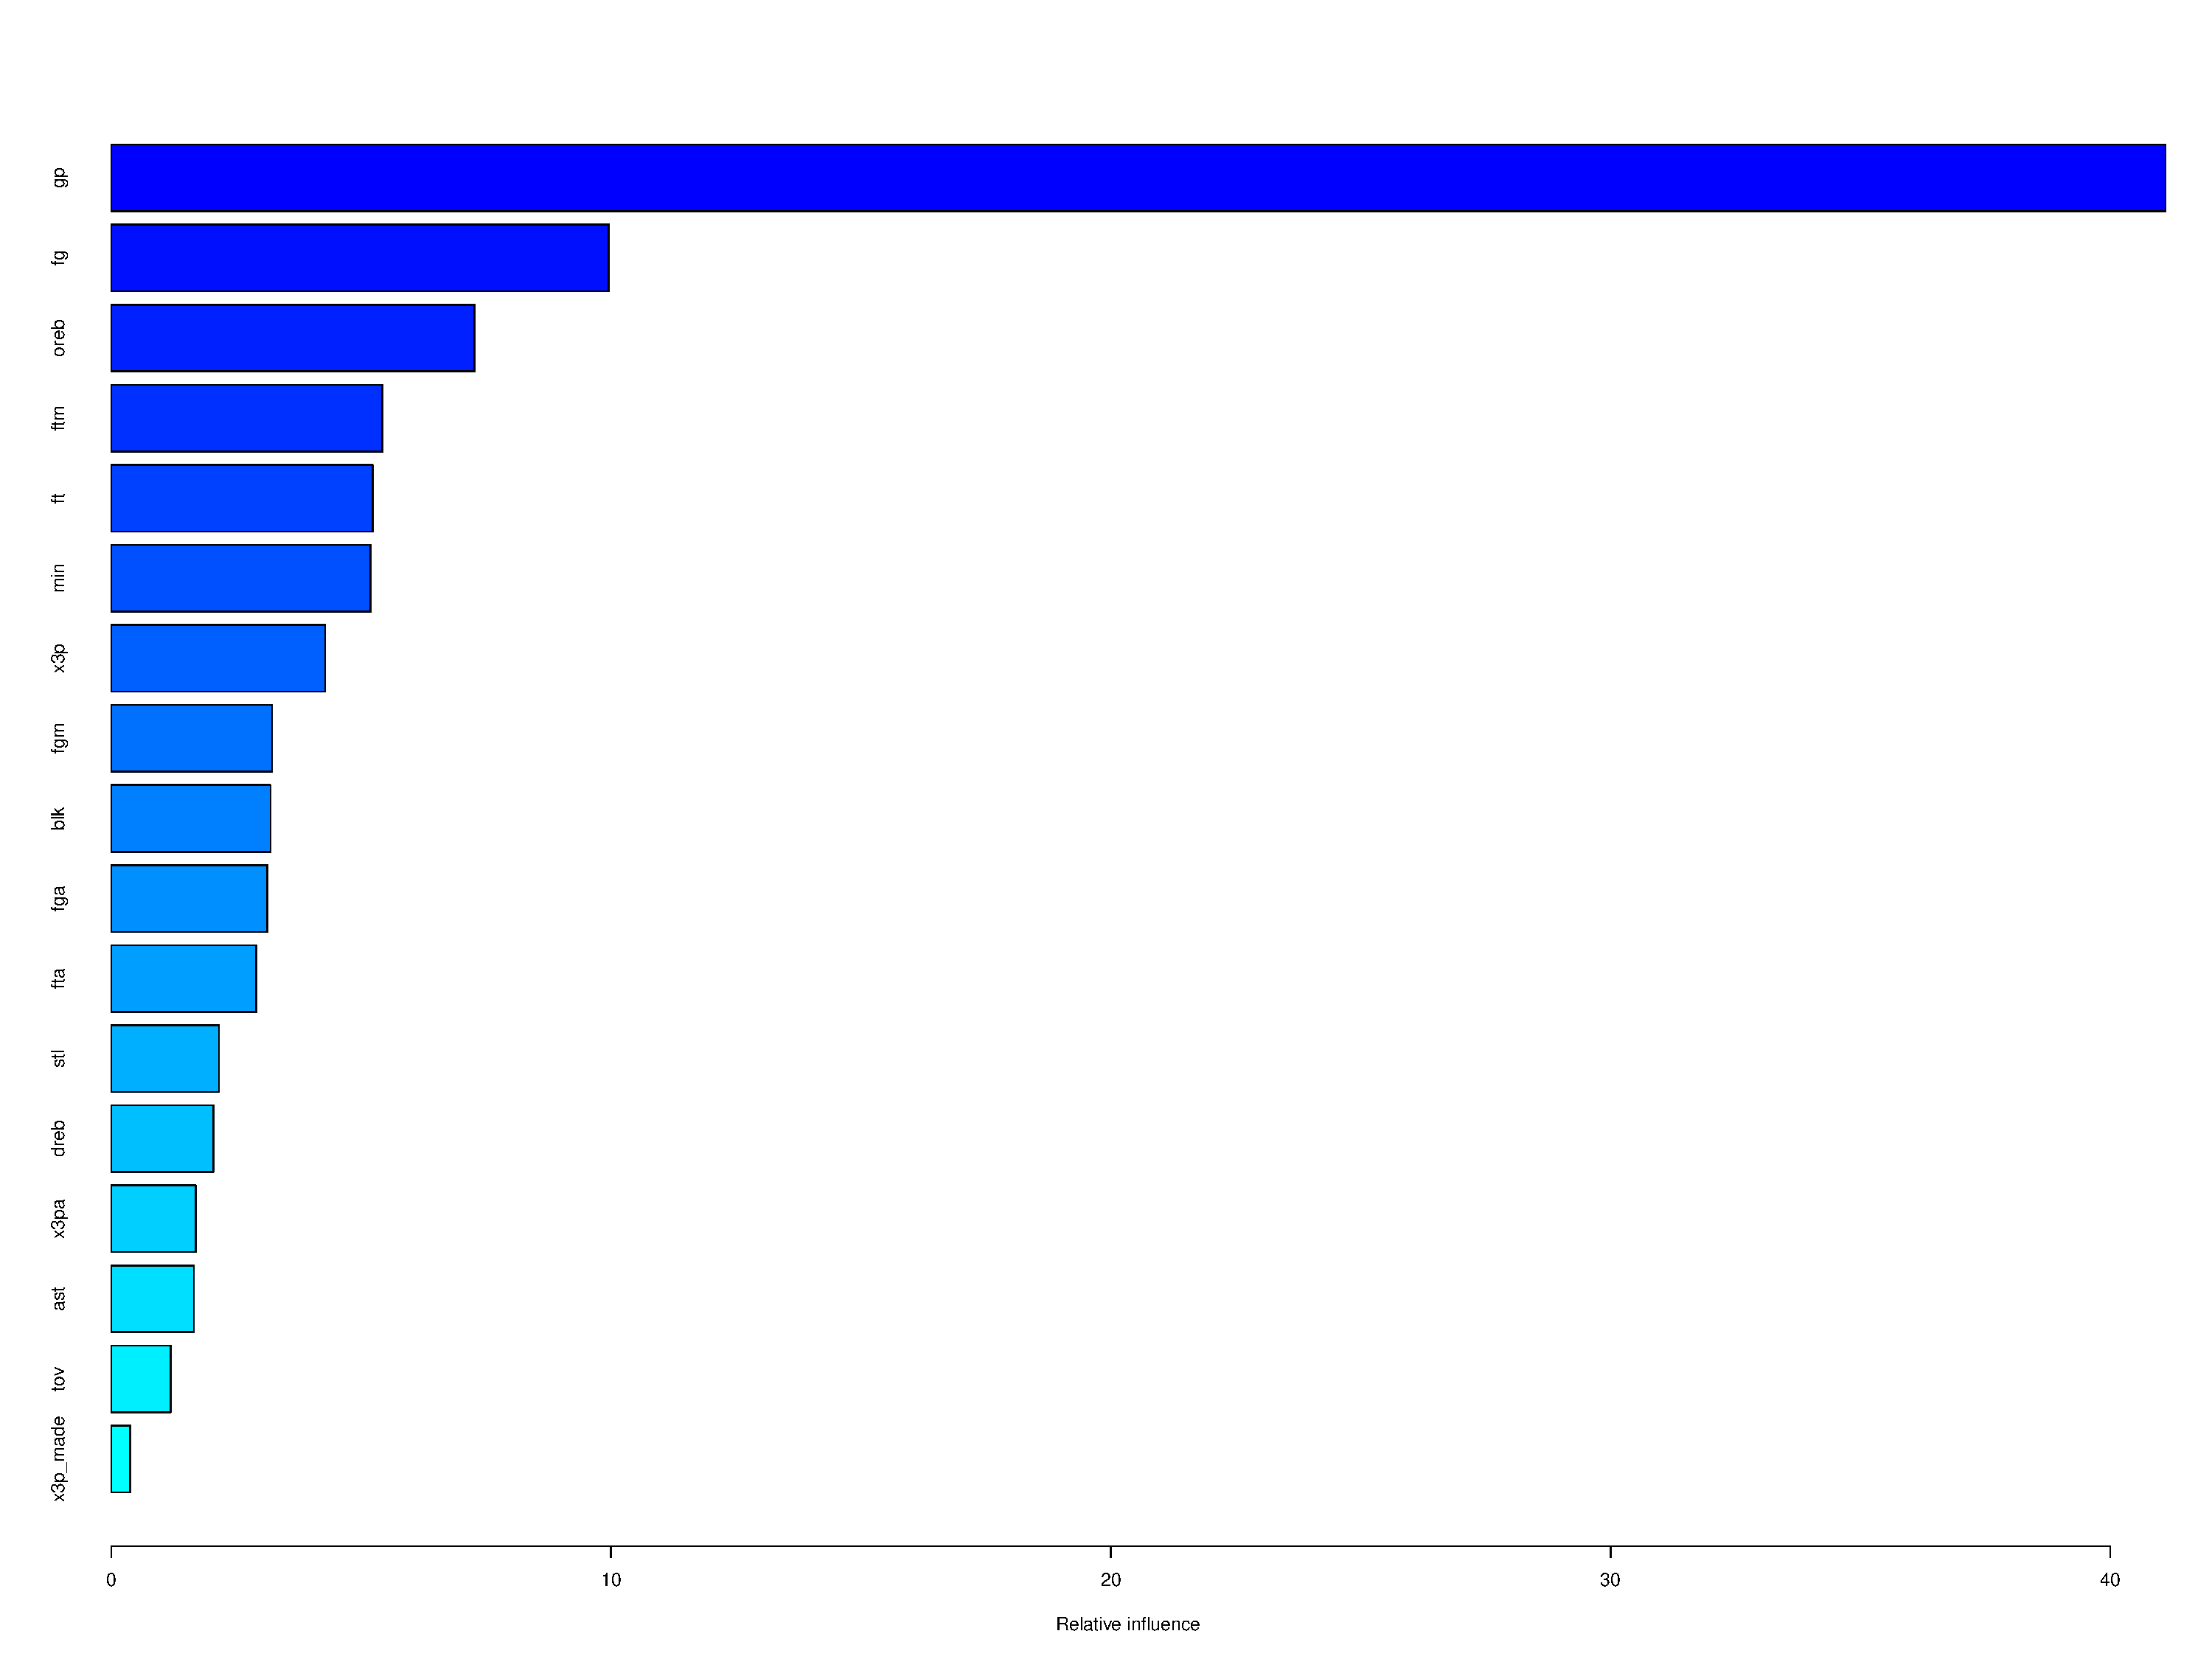
\includegraphics[width=0.8\linewidth]{ImageFiles/Classification/Trees/boost_4_rel_inf_best.pdf}
		\caption{}
		\label{fig:boost_4_rel_inf}
	\end{subfigure}%
	\hfill
	\begin{subtable}{0.5\textwidth}
		\centering
		\begin{tabular}{|| cr | cc ||}    
			\hline
			\multicolumn{2}{|c|}{Prediction} 
			& 0 & 1 \\
			\hline
			\hline
			& 0 & 67 & 46 \\
			& 1 & 51 & 156 \\
			\hline
		\end{tabular}
		\caption{}
		\label{table:ConfMaBoost}
	\end{subtable}
	\caption{Plot of the main results from the boosting technique, taking the model of the best iteration (the one with the minimum cross-validation error). (a) Boosting relative influence of each variable: it provides insights about the key contributors to the model's performance. (b) Confusion matrix of the boosting model.}
	\label{BoostRes}
\end{figure}

As with the previous models, the most significant regressor is still ``GP''. However, based on the confusion matrix in \Tab~\ref{table:ConfMaBoost}, it results that there is no improvement in accuracy. Therefore, using Boosting is not recommended, since it would just lead to interpretability loss.

